\documentclass[12pt]{article}


\usepackage[
    a4paper, 
    margin=2.5cm]{geometry}
\usepackage[utf8]{inputenc}         % UTF8 enkodiranje
\usepackage[slovene]{babel}         % Slovenščina
\usepackage[
    pdfusetitle, 
    hidelinks, 
    unicode]{hyperref}              % Nastavi atribute PDF-ja, ne označuj povezav
\usepackage{microtype}              % Izboljšave za tipografijsko perfekcijo :)
\usepackage{enumitem}               % Seznami za člene
\usepackage{graphicx}               % Vključitev slik
\usepackage{dirtytalk}              % Citat
\usepackage{listings}               % Kodni blok
\usepackage{fancyvrb}
\usepackage[font=]{caption}         % Required for specifying captions
\usepackage[normalem]{ulem}         % Krašanje enot v enačbi
\usepackage{times}                  % Times New Roman pisava
\usepackage{tikz} 
\usepackage[european]{circuitikz}   % Električna vezja
\usepackage{datetime}               % Datum
\usepackage{siunitx}                % tabele
% \usepackage[slovenian]{csquotes}
\usepackage{braket}
\usepackage{amsmath}                % matematika ki izgleda lepo
\usepackage{amsfonts}               % množice
\usepackage{longtable}              % več vrstic v tabeli
\usepackage[style=ieee, maxbibnames=3, minbibnames=1, 
    maxcitenames=1, mincitenames=1, sorting=nyt]{biblatex}   % Navajanje virov
\bibliography{viri}

\urlstyle{rm}

\setlength{\parindent}{0em}
\setlength{\parskip}{1ex}

\setcounter{secnumdepth}{5}
\setcounter{tocdepth}{4}

\renewcommand{\thesection}{\arabic{section}}
\renewcommand{\thesubsection}{\thesection.\arabic{subsection}}
\renewcommand{\thesubsubsection}{\thesubsection.\arabic{subsubsection}}
\renewcommand{\theparagraph}{\thesubsubsection.\arabic{paragraph}}
\renewcommand{\thesubparagraph}{\theparagraph.\arabic{subparagraph}}

\renewcommand{\labelnamepunct}{\addcomma\space}
\DeclareFieldFormat[article]{title}{#1}
\DeclareFieldFormat[online]{title}{\mkbibemph{#1}}

\DefineBibliographyStrings{slovene}{
  andothers = {et. al\adddot},
  urlseen = {dostopano:}
}

\newdateformat{MMYYYYdate}{\monthname[\THEMONTH] \THEYEAR}

\title{Obrestni račun}
\author{Jaka Kovač, G 4. b}

\begin{document}
\pagenumbering{arabic}

\begin{center}
    \thispagestyle{empty}
    
\includegraphics[scale=1]{slike/logotip_vegova_leze_brezokvirja.png}
    \\
    \textbf{Vegova ulica 4, 1000 Ljubljana}

    \vspace{\fill} 
    Seminarska naloga pri predmetu matematika

    \Huge{\textbf{Obrestni račun}}

    \normalsize
    \vspace{\fill}

    Mentor: Karin Kastelic, prof. mat., spec. \hfill Avtor: Jaka Kovač, G 4. b\\
    \null
    Ljubljana, oktober 2023 – \MMYYYYdate\today 
\end{center}
\newpage
\thispagestyle{empty}
\null
\newpage

\section*{Povzetek}
V tej seminarski nalogi bom predstavil obrestni rečun in njegove vrste ter primere uporabe.
\\ %prazna vrstica
\textbf{Ključe besede:} obrestni račun, obrestna mera, anuiteta, amortizacijski načrt

\vfill
\section*{Abstract}
\foreignlanguage{english}{This paper describes mathematics behind interest rates and their
usecases.
\\ %prazna vrstica
\textbf{Keywords:} (compound) interest rate, annuity, amortization schedule}
\vfill

% KAZALO 
\newpage
\thispagestyle{empty} % ne številčimo strani
\tableofcontents % kazalo
\listoffigures   % kazalo slik
\listoftables    % kazalo tabel

\newpage
\section{Uvod}
Že od nekdaj so ljudje med seboj trgovali. Včasih so med sabo menjali dobrine (naturalno 
gospodarstvo), ko pa so okoli leta 3000 pr. n. št. v Mezopotamiji \cite{wiki:money} pričeli
z menjavo izdelkov za denar. Izumu denarja so botrovale tudi banke. Posojanje denarja v 
zameno za več denarja se sprva zdi precej nenavadno, vendar pa je to le ena izmed storitev
modernejšega sveta. 

\section{Teorija}
    \subsection{Pojmi, definicije in uporabljeni simboli}
        \begin{table}[h!]
            \centering
            \begin{tabular}{|c|c|c|p{7cm}|}
                \hline
                \textbf{simbol} & \textbf{pojem} & \textbf{enota} & \textbf{definicija} \\ \hline
                $G_0$ & glavnica                & EUR    & denarna vrednost, ki si jo od nekoga izposodimo ali jo mi posodimo nekomu \\ \hline 
                $o$   & obresti                 & EUR    & nadomestilo ali odškodnina za izposojeni denar, ker le-ta v času obrestovanja ni na voljo lastniku \\ \hline
                $p$   & obrestna mera           & \%     & obresti podane v odstodkih (navadno \textbf{letna obrestna mera}) \\ \hline
                $p_k$ & konformna obrestna mera & \%     & obrestna mera, ki se uporablja za izračun obresti v posebnih primerih \ref{konformna} \\ \hline
                $r$   & obrestovalni faktor     &        & $$r = 1 + \frac{p}{100}$$ \\ \hline
                $r_k$ & konformni obrestovalni faktor &  & $$r_k = 1 + \frac{p_k}{100}$$ \\ \hline
                $k$   & število kapitalizacijskih odbobji &  & kolikokrat smo izračunali obresti \\ \hline
                $c$   & anuiteta                & EUR    & redno odplačilo \\ \hline
            \end{tabular}

            \medskip
            \centering povteto po \cite{vega4}
            \caption{Simboli, pojmi in njihove definicije}
            \label{tab:simboli}
        \end{table}

        \subsubsection{Prikazovanje podatkov v tabelah in izračunih}
        Zaradi preprostosti prikazavanja so denarne vrednosti zaokrožene na cente natačno
        in prikazane v EUR. Številčne vrednosti so zaokrožene na 3 od 0 različna decimalna 
        mesta. V izračunih se uporablja dejanska vrednost. Ničto leto označuje polog denarja,
        prikazane vrednosti pa stanje ob koncu leta razen kjer je navedeno drugače. 
    \subsection{Obrestovanje}
        \subsubsection{Navadno obrestovanje}
        Navadno obrestovanje je način obrestovanja, kjer so obresti odvisne le od glavnice
        in obrestne mere, ne pa tudi od prejšnjih obresti. Končna vrednost glavnice po $n$
        letih se izračuna po formuli:
        \begin{equation}
            G_n = G_0 \cdot (1 + \frac{p*n}{100})
        \end{equation}

        Vzemimo primer, kjer na banko položimo 10 000 € za 5 let pri 5\% letni obrestni meri. 
        \begin{center}
            \begin{table}[h!]
                \centering
                \begin{tabular}{|c|c|}
                    \hline
                    \textbf{leto} & \textbf{vrednost [EUR]} \\ \hline
                    0 & 10 000,00 \\ \hline
                    1 & 10 500,00 \\ \hline
                    2 & 11 000,00 \\ \hline
                    3 & 11 500,00 \\ \hline
                    4 & 12 000,00 \\ \hline
                    5 & 12 500,00 \\ \hline
                \end{tabular}
                \caption{Navadno obrestovanje}
            \end{table}
        \end{center}

        \subsubsection{Obrestno obrestovanje}
        Obrestno obrestovanje je način obrestovanja, kjer so obresti odvisne tako od 
        glavnice, obrestne mere in prejšnjih obresti. Vsota glavnice in obresti torej 
        postne glavnica za naslednje kapitalizacijsko obdobje. Končna vrednost glavnice 
        po $n$ letih se izračuna po formuli:
        \begin{equation}
            G_n = G_0 \cdot r^n
        \end{equation}

        Obrestovalni faktor $r$ izračunamo po formuli:
        \begin{equation}
            r = 1 + \frac{p}{100}
        \end{equation}
        
        Enotna formula za izrčun vrdnosti glavnice:
        \begin{equation}
            G_n = G_0 \cdot (1 + \frac{p}{100})^n
        \end{equation}

        \newpage
        Za primer vzemimo enake podatke kot pri navadnem obrestovanju.
        \begin{center}
            \begin{table}[h!]
                \centering
                \begin{tabular}{|c|c|c|c|}
                    \hline
                    \textbf{leto} & \textbf{letne obresti [EUR]} & \textbf{skupne obresti [EUR]} & \textbf{vrednost [EUR]} \\ \hline
                    0 & N/A & N/A & 10 000,00 \\ \hline
                    1 & 500,00 & 500,00 & 10 500,00 \\ \hline
                    2 & 525,00 & 1 025,00 & 11 025,00 \\ \hline
                    3 & 551,25 & 1 576,25 & 11 576,25 \\ \hline
                    4 & 578,81 & 2 155,06 & 12 155,06 \\ \hline
                    5 & 636,69 & 2 762,82 & 12 762,82 \\ \hline
                \end{tabular}
                \caption{Obrestno obrestovanje}
            \end{table}
        \end{center}

    \subsection{Obrestna mera}
        \subsubsection{Relativna obrestna mera}
        Če je v enem letu več kapitalizacijskih obdobji, nam pa je podana letna obrestna 
        mera si lahko s formulo \eqref{rom} izračunamo obrestno mero, ki se dejansko 
        uporabi za izračun obresti na koncu vsakega kapitalizacijskega obdobja.

        \begin{equation}
            p(k) = \frac{p(letna)}{k}
            \label{rom}
        \end{equation}

        Formula za obrestovalni faktor je:
        \begin{equation}
            \begin{split}
                r & = 1 + \frac{p(k)}{100} \\
                r & = 1 + \frac{\frac{p(letna)}{k}}{100} \\
                r & = 1 + \frac{p(letna)}{k \cdot 100}
            \end{split}
        \end{equation}

        s tem pa je enačba za izračun glavnice po $k$ kapitalizacijskih obdobjih 
        ($k = k(letno) \cdot n$):
        \begin{equation}
            \begin{split}
                G_n & = G_0 \cdot r^k \\
                G_n & = G_0 \cdot (1 + \frac{p(na \: kapitalizacijsko \: obdobje)}{100 \cdot k})^k
            \end{split}
        \end{equation}


        \begin{longtable}{|c|c|c|c|c|}
            \hline
            \textbf{leto} & \textbf{četrtletje} & \textbf{$k$} & \textbf{letno [EUR]} & \textbf{četrtletno [EUR]} \\ \hline
            \endfirsthead
            \endhead
            0 & 0  & 0   & 10000,00 & 10000,00 \\ \hline \hline
            1 & 1  & 1   & 10000,00 & 10125,00 \\ \hline
              & 2  & 2   & 10000,00 & 10251,56 \\ \hline
              & 3  & 3   & 10000,00 & 10379,71 \\ \hline
              & 4  & 4   & 10500,00 & 10509,45 \\ \hline \hline
            2 & 1  & 5   & 10500,00 & 10640,82 \\ \hline 
              & 2  & 6   & 10500,00 & 10773,83 \\ \hline
              & 3  & 7   & 10500,00 & 10908,50 \\ \hline
              & 4  & 8   & 11025,00 & 11044,86 \\ \hline \hline
            3 & 1  & 9   & 11025,00 & 11182,92 \\ \hline 
              & 2  & 10  & 11025,00 & 11322,71 \\ \hline
              & 3  & 11  & 11025,00 & 11464,24 \\ \hline
              & 4  & 12  & 11576,25 & 11607,55 \\ \hline \hline
            4 & 1  & 13  & 11576,25 & 11752,64 \\ \hline 
              & 2  & 14  & 11576,25 & 11899,55 \\ \hline
              & 3  & 15  & 11576,25 & 12048,29 \\ \hline
              & 4  & 16  & 12155,06 & 12198,90 \\ \hline \hline
            5 & 1  & 17  & 12155,06 & 12351,38 \\ \hline 
              & 2  & 18  & 12155,06 & 12505,77 \\ \hline
              & 3  & 19  & 12155,06 & 12662,10 \\ \hline
              & 4  & 20  & 12762,82 & 12820,37 \\ \hline
            \caption{Četrtletno obrestno obrestovanje}
        \end{longtable}

        \paragraph{Eulerjevo število}
            \label{euler}
            Opazimo lahko, da smo z obrestovanjem na koncu vsakega četrtletja pridobili več obresti
            kot pri obrestovanju letno. Od tod izvira tudi Eulerjevo število $e$, ki predstavlja
            100 \% obrestno mero. Če imamo v enem letu neskončno kapitalizacijskih obdobji,
            predstavlja število $e$ obrestovalni faktor, če bi ekvivalentne obresti računali letno.
            Izračunamo ga lahko po formuli: \hfill \cite{wiki:euler}
            \begin{equation}
                e = \lim_{k \to \infty} (1 + \frac{1}{k})^k
            \end{equation}

        \subsubsection{Konformna obrestna mera}
        \label{konformna}
        Konformna obrestna mera je obrestna mera, ki se uporablja za izračun obresti, ko
        banka letno obrestno mero preračuna na več kapitalizacijskih obdobji letno tako, da
        je skupna vrednost obresti enaka kot če bi obrestovali letno.
        
        \begin{equation}
            \begin{split}
                G_n = G_0 \cdot r & = G_0 \cdot r_k^k \\
                r & = r_k^k \\
                r_k & = \sqrt[k]{r} \\
                1 + \frac{p_k}{100} & = \sqrt[k]{1 + \frac{p}{100}} \\
                p_k & = 100 \cdot (\sqrt[k]{1 + \frac{p}{100}} - 1)
            \end{split}
        \end{equation}

        Konformni obrestovalni faktor:
        \begin{equation}
            \begin{split}
                r_k & = 1 + \frac{p_k}{100} \\
                r_k & = 1 + \frac{100 \cdot (\sqrt[k]{1 + \frac{p}{100}} - 1)}{100} \\
                r_k & = \sqrt[k]{1 + \frac{p}{100}}
            \end{split}
        \end{equation}

        Ob prejšnjem primeru vzemimo, da nam banka izračuna obresti na vsako četrtletje,
        vendar pri tem uporabijo konformno obrestno mero.

        Izračun konformne obrestne mere:
        \begin{equation}
            \begin{split}
                p_k & = 100 \cdot (\sqrt[k]{1 + \frac{p}{100}} - 1) \\
                p_k & = 100 \cdot (\sqrt[4]{1 + \frac{5}{100}} - 1) \\
                p_k & \approx 1.22
            \end{split}
        \end{equation}

        in izračun konformnega obrestovalnega faktorja:
        \begin{equation}
            \begin{split}
                r_k & = \sqrt[k]{1 + \frac{p}{100}} \\
                r_k & = \sqrt[4]{1 + \frac{5}{100}} \\
                r_k & \approx 1.01
            \end{split}
        \end{equation}

        \begin{longtable}{|c|c|c|c|c|}
            \hline
            \textbf{leto} & \textbf{četrtletje} & \textbf{k} & \textbf{letno [EUR]} & \textbf{četrtletno [EUR]} \\ \hline
            \endfirsthead
            %
            \endhead
            %
            0 & 0 & 0  & 10000,00  & 10000,00  \\ \hline \hline
            1 & 1 & 1  & 10500,00  & 10122,72  \\ \hline
              & 2 & 2  & 10500,00  & 10246,95  \\ \hline
              & 3 & 3  & 10500,00  & 10372,70  \\ \hline
              & 4 & 4  & 10500,00  & 10500,00  \\ \hline \hline
            2 & 1 & 5  & 11025,00  & 10628,86  \\ \hline
              & 2 & 6  & 11025,00  & 10759,30  \\ \hline
              & 3 & 7  & 11025,00  & 10891,34  \\ \hline
              & 4 & 8  & 11025,00  & 11025,00  \\ \hline \hline
            3 & 1 & 9  & 11576,25  & 11160,30  \\ \hline
              & 2 & 10 & 11576,25  & 11297,26  \\ \hline
              & 3 & 11 & 11576,25  & 11435,91  \\ \hline
              & 4 & 12 & 11576,25  & 11576,25  \\ \hline \hline
            4 & 1 & 13 & 12155,06  & 11718,32  \\ \hline
              & 2 & 14 & 12155,06  & 11862,13  \\ \hline
              & 3 & 15 & 12155,06  & 12007,70  \\ \hline
              & 4 & 16 & 12155,06  & 12155,06  \\ \hline \hline
            5 & 1 & 17 & 12762,82  & 12304,23  \\ \hline
              & 2 & 18 & 12762,82  & 12455,23  \\ \hline
              & 3 & 19 & 12762,82  & 12608,09  \\ \hline
              & 4 & 20 & 12762,82  & 12762,82  \\ \hline
              \caption{Četrtletno obrestno obrestovanje s konformno obrestno mero}
        \end{longtable}
        % tuki dodej grafe če boš meu cajt

    \subsection{Krediti}
    Do sedaj smo obravnavali le obrestovanje na depozite, kjer smo mi banki posodili denar.
    Krediti so v osnovi precej podobni, le da sta vlogi obrnjenji, saj banka nam posodi
    denar, mi pa ga moramo z obrestmi vrniti.

    Ko pri banki zaprosimo za kredit, nam ponavadi pošljejo amortizacijski načrt, ki nam
    pove koliko moramo plačati vsak mesec in koliko denarja bomo plačali skupaj. Navadno
    vsebuje podatke o mesečnem obroku (anuiteti), obrestih, razdolžnini in 
    stanju dolga. 
    $$\text{ANUITETA} = \text{OBRESTI} + \text{RAZDOLŽNINA}$$
    Privzemimo, da smo si na banki izposodili $G_n$ denarja. Z banko se dogovorimo, da bomo
    kredit vrnili z $n$ letnimi anuitetami, kjer prvo anuiteto vrnemo čez eno leto. Banka
    uporablja letno kapitalizacijo, letna obrestna mera a je $p$. Anuiteta $G_0$ je torej:
    
    \begin{equation}
        \begin{split}
            G_n \cdot r^n & = G_0 \cdot r^{n - 1} + G_0 \cdot r^{n - 2} + \cdots + G_0 \cdot r + G_0 \\
            G_n \cdot r^n & = G_0 \cdot (r^{n - 1} + r^{n - 2} + \cdots + r + 1) \\
            G_n \cdot r^n & = G_0 \cdot \frac{r^n - 1}{r - 1} \\
            \frac{G_n \cdot r^n}{G_0} & = \frac{r^n - 1}{r - 1} \\
            \frac{G_0}{G_n \cdot r^n} & = \frac{r - 1}{r^n - 1} \\
            G_0 & = \frac{G_n \cdot r^n \cdot (r - 1)}{r^n - 1} \\
        \end{split}
    \end{equation}

    Za primer vzemimo kredit v višini 150 000 € za 20 let pri 4\% letni obrestni meri. 
    \begin{equation}
        \begin{split}
            G_0 & = \frac{G_n \cdot r^n \cdot (r - 1)}{r^n - 1} \\
            G_0 & = \frac{150 \enskip 000 \text{ €} \cdot 1.04^{20} \cdot (1.04 - 1)}{1.04^{20} - 1} \\
            G_0 & \approx 11 \enskip 037.26 \text{ €}
        \end{split}
    \end{equation}

    Izračunali smo torej, da bomo naslednjih 20 let plačevali 11 037,26 € letno. Ker bomo
    banki vsako leto manj dolžni, bodo naše obresti manjše (kar si v tem primeru želimo)
    hkrati pa bo večja razdolžnina (delež dolga, ki ga odplačamo). 
    
    Izdelajmo amortizacijski načrt:
    \begin{longtable}{|c|c|c|c|c|}
        \hline
        \textbf{leto}   & \textbf{anuiteta [EUR]}  & \textbf{obresti [EUR]}  & \textbf{razolžnina [EUR]} & \textbf{dolg [EUR]} \\ \hline
        \endfirsthead
        %
        \endhead
        %
        0      & /          & /         & /          & 150 000,00 \\ \hline
        1      & 11 037,26  & 6 000,00  & 5 037,26   & 144 962,74 \\ \hline
        2      & 11 037,26  & 5 798,51  & 5 238,75   & 139 723,98 \\ \hline
        3      & 11 037,26  & 5 588,96  & 5 448,30   & 134 275,68 \\ \hline
        4      & 11 037,26  & 5 371,03  & 5 666,24   & 128 609,45 \\ \hline
        5      & 11 037,26  & 5 144,38  & 5 892,88   & 122 716,56 \\ \hline \hline 
        6      & 11 037,26  & 4 908,66  & 6 128,60   & 116 587,96 \\ \hline
        7      & 11 037,26  & 4 663,52  & 6 373,74   & 110 214,22 \\ \hline
        8      & 11 037,26  & 4 408,57  & 6 628,69   & 103 585,52 \\ \hline
        9      & 11 037,26  & 4 143,42  & 6 893,84   & 96 691,68  \\ \hline 
        10     & 11 037,26  & 3 867,67  & 7 169,60   & 89 522,09  \\ \hline \hline
        11     & 11 037,26  & 3 580,88  & 7 456,38   & 82 065,71  \\ \hline
        12     & 11 037,26  & 3 282,63  & 7 754,63   & 74 311,07  \\ \hline
        13     & 11 037,26  & 2 972,44  & 8 064,82   & 66 246,25  \\ \hline
        14     & 11 037,26  & 2 649,85  & 8 387,41   & 57 858,84  \\ \hline
        15     & 11 037,26  & 2 314,35  & 8 722,91   & 49 135,93  \\ \hline \hline
        16     & 11 037,26  & 1 965,44  & 9 071,83   & 40 064,11  \\ \hline
        17     & 11 037,26  & 1 602,56  & 9 434,70   & 30 629,41  \\ \hline
        18     & 11 037,26  & 1 225,18  & 9 812,09   & 20 817,32  \\ \hline
        19     & 11 037,26  & 832,69    & 10 204,57  & 10 612,75  \\ \hline
        20     & 11 037,26  & 424,51    & 10 612,75  & 0,00       \\ \hline \hline
        SKUPAJ & 220 745,25 & 70 745,25 & 150 000,00 &            \\ \hline
        \caption{Amortizacijski načrt}
    \end{longtable}

    Iz načrta je razvidno, da prvih nekaj obrokov plačujemo obresti, nato pa se obresti
    zmanjšujejo, razdolžnina pa povečuje. V zadnjih letih večinsko plačujemo le še razdolžnino.

    To je sicer odvisno od banke, vendar se pogosto splača kredit odplačevati predčasno, saj
    se po plačanih obresith ves znesek prišteje razolžnini. 
    \newpage

\section{Avtentični primer}
    Na Delavsko hranilnico, d. d. sem želel položiti 10 000 € za 20 let (dolgoročno varčevanje).
    Ponujena letna obrestna mera je 2,7 \%. \\

    \begin{figure}[h!]
        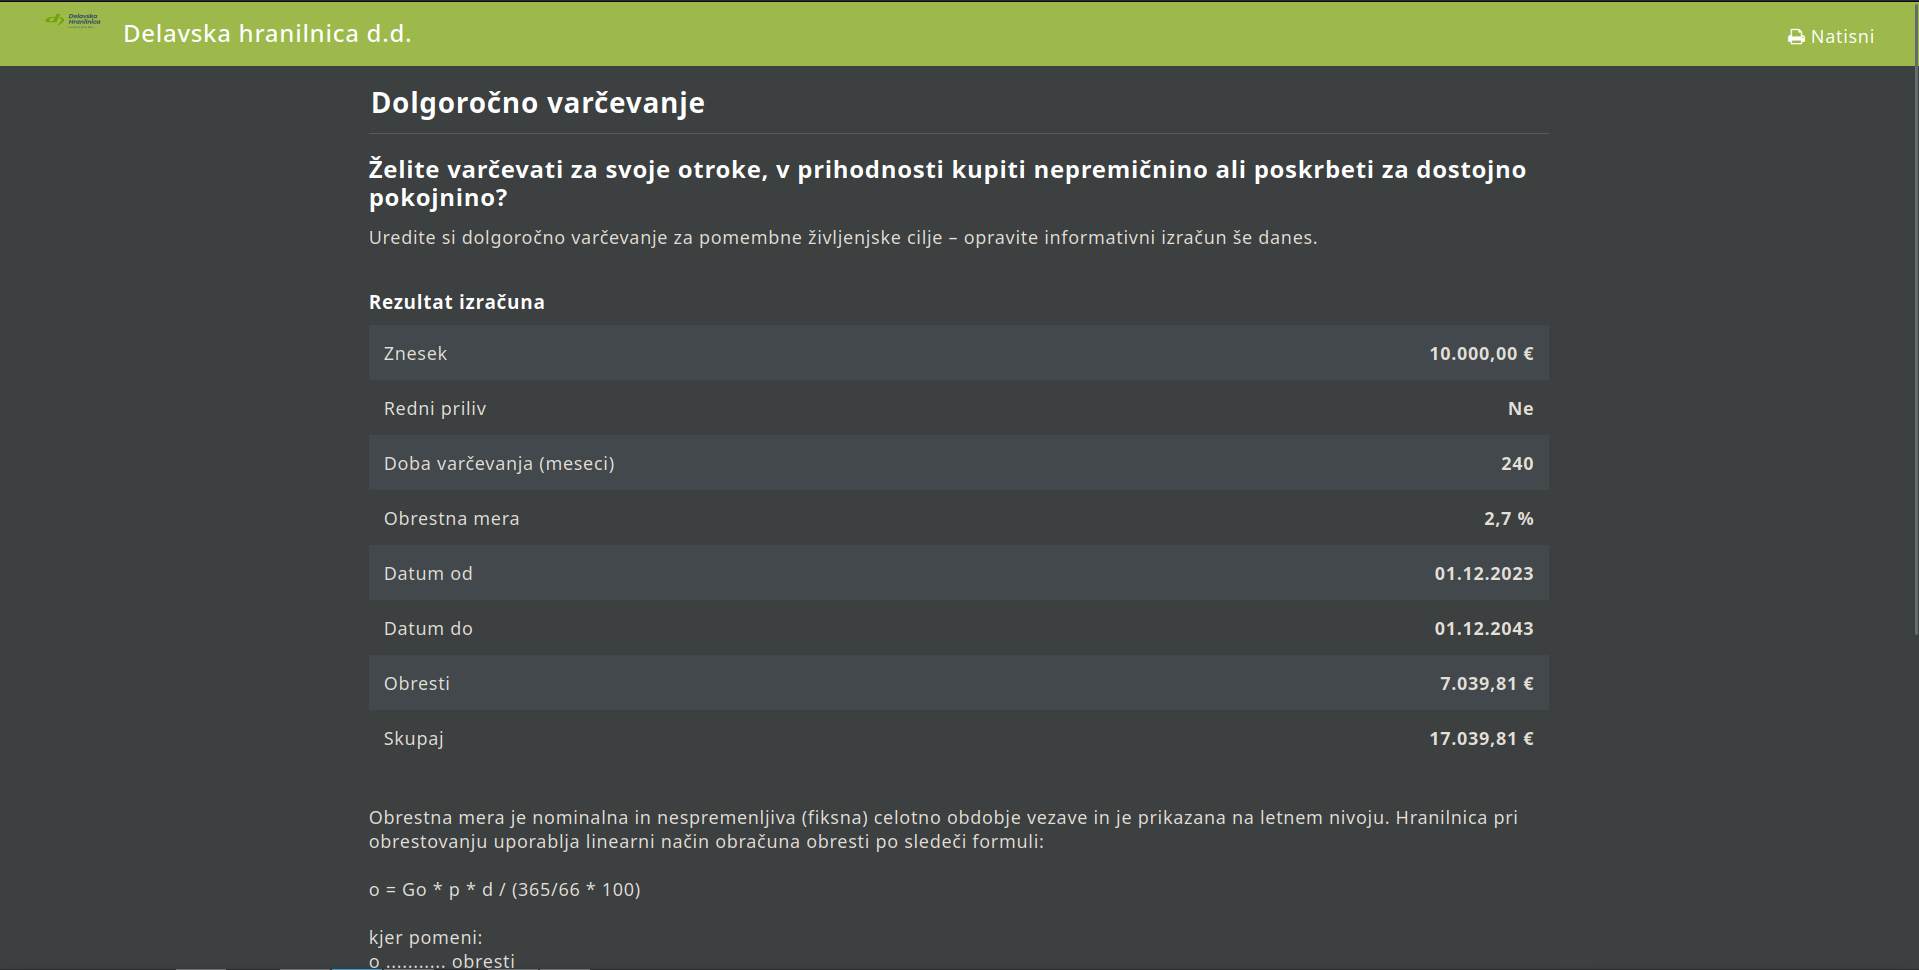
\includegraphics[width=\textwidth]{slike/2023-11-28_18-36.png}
        \caption{Ponudba Delavske hranilnice, d. d.; vir: \cite{DH}}
    \end{figure}

    Opazimo lahko, da nam ponujajo obrestno obrestovanje. Preverimo če naše enačbe res držjo.

    \begin{equation}
        \begin{split}
            G_n & = G_0 \cdot (1 + \frac{p}{100})^n \\
            G_n & = 10 \enskip 000 \text{ €} \cdot (1 + \frac{2,7}{100})^{20} \\
            G_n & = 10 \enskip 000 \text{ €} \cdot 1,027^{20} \\
            G_n & = 10 \enskip 000 \text{ €} \cdot 1,70 \\
            G_n & \approx 17 \enskip 037,62 \text{ €}
        \end{split}
    \end{equation}

    Vidimo, da pri izračunu pride do manjše napake (0,19 €) verjetno zaradi zaokroževanja,
    saj nam banka obresti izračuna vsako leto, pri tem pa necele vrednosti zaokroži.

    \newpage

\section{Ugotovitve}
    \begin{itemize}
        \item Obrestno obrestovanje se nam bolj splača kot navadno obrestovanje. Prav tako nam
        krajša kapitalizacijska doba prinese več dobička. V poglavju \ref{euler} smo spoznali
        da je ob dani obrestni meri izkupiček največji pri neskončno kratki kapitalizacijsk dobi.
        \item Ob avtentičnem primeru smo videli, da nam tudi banka občasno "po nesreči" doda
        manjšo količino denarja. To se verjetno zgodi le ob napakah zaokroževanja, ki pa se lahko 
        pri obrestnem obrestovanju hitro naberejo.
        \item \LaTeX je čudovito orodje, ki močno poenostavi pisanje tokumentov z matematičnimi
        izrazi. Če želiš uporabljati git (orodje za nadzor inaičic) se (\LaTeX) bolje obnese kot Word,
        ker je .docx v bistvu binarna datoteka, standard pa ni javno objavljen.
    \end{itemize}

\newpage
\section{Zaključek}
    Med pisanjem seminarske naloge sem se učil o računanju obresti. To znanje, mi bo koristilo
    ko bo v ne tako zelo daljni prihodnosti želel pridobiti kredit za stanovanje ali hišo.
    Morda pa bom že kmalu pričel z varčevanjem denarja in kredita sploh ne bom potreboval. 



\newpage
\begingroup
\makeatletter
    \section{Viri in literatura}
    \nocite{*}
    \printbibliography[heading=none]
\makeatother
\endgroup
\newpage

\begin{samepage}
    \thispagestyle{empty}
    \section*{Izjava o avtorstvu}
    Izjavljam, da je seminarska naloga v celoti moje avtorsko delo, ki sem ga 
    izdelal samostojno s pomočjo navedene literature in pod vodstvom mentorja.

    \vfill
    
    \today \hfill Jaka Kovač, G 4. b
    
    \vspace{3 cm}
\end{samepage}

\end{document}
